\subsection{Fonctionnement général}
Le projet, comme évoqué précédemment, s'articule autour de deux parties : le plugin \texttt{Inkscape} et les algorithmes.\\

Le plugin \texttt{Inkscape}, décrit plus en détail par la suite, envoie à un script Python un certain nombre d'arguments bruts. Ce dernier est chargé d'interpréter les arguments d'Inkscape et de les convertir (notamment au niveau des unités) en un format accepté par notre programme, qu'il appelle avec ces nouveaux arguments.

Ce programme, le solveur reçoit un fichier \texttt{SVG} et les arguments, et renvoie un fichier  \texttt{SVG} résultat sur la sortie standard, qui est alors affiché par \texttt{Inkscape}.\\

La partie la plus importante du projet est ce programme, dont nous allons par la suite détailler l'architecture. Un diagramme de classe de ce programme est visible en figure~\ref{fig:diagramme}

\begin{figure}[!htb]
\centering
\includegraphics[scale=0.7]{img/ClassDiagram.png}
\caption{Diagramme de classe du programme principal}
\label{fig:diagramme}
\end{figure}

\subsection{Concept de Shape}

Nous introduisons le concept de \texttt{Shape} (forme), que nous utiliserons par la suite. Il s'agit d'une classe représentant une forme interpolée. Elle peut représenter un ou plusieurs polygones non indépendants, potentiellement chacun composés de trous. En effet, cette classe contient un \texttt{MultiPolygon}, type de la librairie Boost, lequel contient plusieurs \texttt{Polygon}. Enfin ce dernier contient un \texttt{Ring} (polygone fermé) décrivant son contour, et potentiellement plusieurs autres décrivant ses trous. Nous verrons dans la partie sur le parseur \texttt{SVG} comment nous transformons le document en un ensemble de telles \texttt{Shapes}. Cette hiérarchie est illustrée en figure~\ref{fig:multipolygon}\\

\begin{figure}[!htb]
\centering
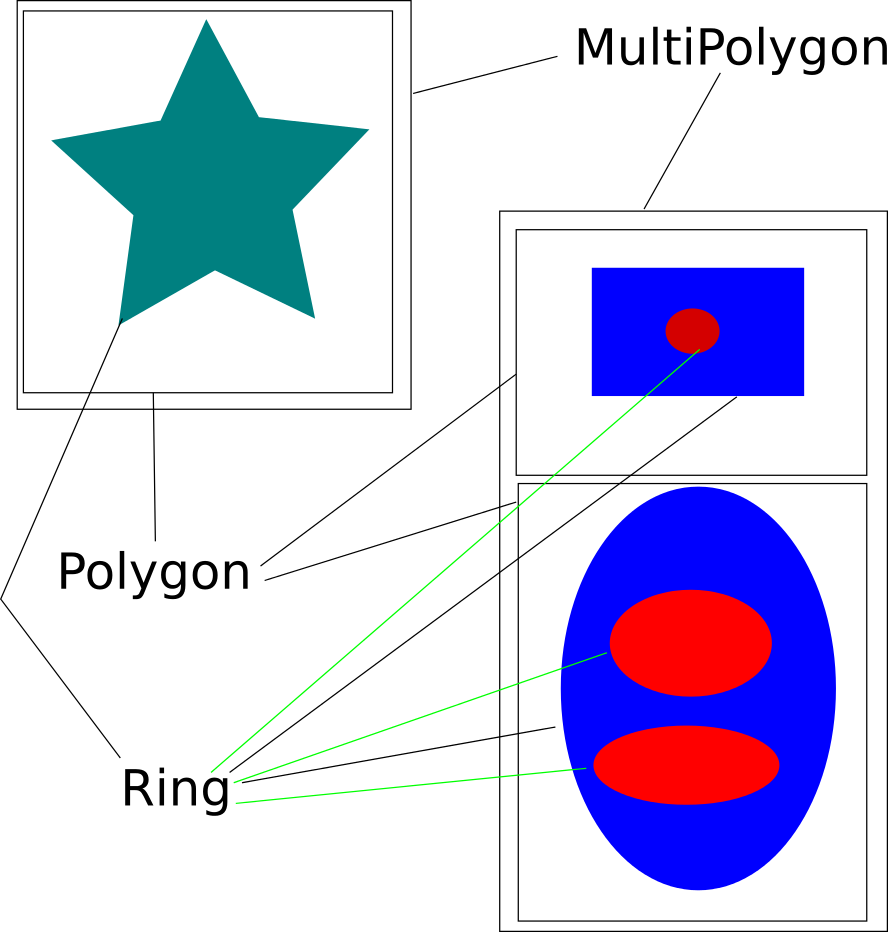
\includegraphics[scale=0.5]{img/MultiPolygon.png}
\caption{Hiérarchie \texttt{MultiPolygon}/\texttt{Polygon}/\texttt{Ring} (vert : \texttt{Ring} interne)}
\label{fig:multipolygon}
\end{figure}

Par la suite, il arrivera que faisions l'union de deux \texttt{Shapes} : il s'agit de générer un unique \texttt{MultiPolygon} contenant les \texttt{Polygons} de la première \textbf{et} la deuxième \texttt{Shape}. On parlera alors de \textit{bloc} de \texttt{Shapes} pour décrire une union (en effet faire l'union de deux \texttt{Shapes} revient à les considérer comme dépendantes l'une de l'autre : elles seront déplacées "ensemble").\\

Toutes ces formes sont stockées dans une classe \texttt{Layout}, qui décrit donc une disposition des pièces à un instant donné.\\

\subsection{Préparation des pièces}

Une fois les pièces générées, on commence par appliquer un \textit{buffer} sur ces dernières, c'est à dire augmenter leur épaisseur dans leur représentation interne. Ceci est utile non seulement pour compenser une erreur potentielle lors de l'interpolation des points, mais aussi si l'utilisateur souhaite une distance minimale entre les pièces une fois le packing réalisé. Le fait d'augmenter l'épaisseur en interne produira ce résultat, puisque les pièces seront positionnées comme si elles étaient plus épaisses, sans augmenter l'épaisseur réelle à la sortie.\\

\subsection{Choix concernant la sortie}

En effet nous avons choisi, lors de la génération du fichier de sortie, de ne pas créer de nouvelles formes à partir de notre représentation interne (potentiellement erronée), mais plutôt d'appliquer des transformations sur les formes originales. De cette manière on conserve l'ensemble des attributs donnés pour l'utilisateur.\\

Cela provoque quelques inconvénients : nous le verrons par la suite dans la classe \texttt{Outer}, mais celà nécessite (à cause de l'utilisation à l'entrée de \texttt{SVG++}) de parcourir une nouvelle fois le fichier original à la sortie.

\subsection{Fonctionnement interne des modules}

\subsubsection{Plug-In}

Afin de gérer l'interface entre Inkscape et notre programme, nous avons implémenté un plug-in python.
Celui-ci s'occupe de récupérer l'ensemble des paramètres transmis par Inkscape. Il effectue également un ensemble d'opérations permettant de convertir les unités de mesure en pixel, qui sont utilisables par notre programme. Il permet notamment d'extraire les dimensiona de la plaque depuis le fichier, puis de les convertir en pixel.\\
Pour réaliser ce travail nous avons utilisé la bibliothèque \texttt{inkex.py} fournie par Inkscape.\\



\subsubsection{Parser et SVG++}
%PARTIE SVG++%
Nous utilisons, pour lire le fichier d'entrée du programme, la bibliothèque \texttt{SVG++}.
Pour utiliser celle-ci, il faut définir un ensemble de comportements à adopter lors de la lecture des balises qui nous intéressent. Les méthodes implémentées au cours du projet sont visibles sur la figure~\ref{fig:SVGPP}.

\begin{figure}[H]
\centering
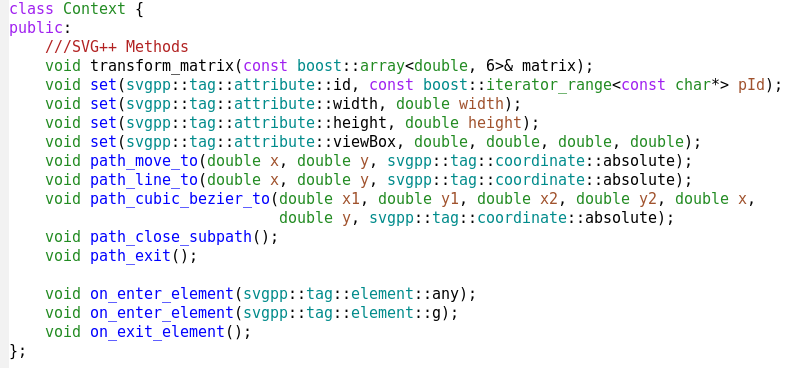
\includegraphics[scale=0.5]{img/SVGPP.png}
\caption{Méthodes à implémenter dans la classe Context de SVG++}
    \label{fig:SVGPP}
\end{figure}

Ces comportements peuvent être généralisés : par exemple, il est possible d'utiliser le comportement des courbes de Bézier sur tout les \texttt{path} rencontrés, la bibliothèque effectue alors la conversion nécessaire pour appliquer le comportement choisi.\\

Ceci permet notamment de ne pas gérer au cas par cas toutes les balises existantes, en ignorant celle n'étant pas utiles pour le bon fonctionnement du programme, et en utilisant un comportement générique pour une certaine variété de balises (\texttt{path}).\\

Cependant, l'implémentation de la bibliothèque est riche en métaprogrammation template.\\
La métaprogrammation est un outil permettant en particulier de générer du code à la compilation, par exemple, il est possible d'écrire une fonction avec un type générique qui sera ensuite déterminé lors de la compilation.\\
Il est également possible de pré-calculer des données lors de la compilation qui seront généralement stockées dans des variables statiques.\\
Ceci permet d'améliorer l'efficacité de certains programmes, et d'écrire du code plus générique. Cependant, les temps de compilations sont plus longs, les métaprogrammes sont assez peu lisibles et, en C++, il est impossible de redéfinir une méthode template dans une classe fille.\\

Il n'est alors pas possible d'utiliser le comportement habituel de la Programmation Orienté Objet (POO) (redéfinition de méthodes dans une classe fille), il est donc nécessaire de préciser quelles méthodes sont implémentées dans un ensemble utilisé par cette bibliothèque.\\
De plus celle-ci ne nous permet pas de stocker le contenu du fichier, nous devons donc ré-effectuer une lecture au moment de la génération du fichier de sortie. Et les temps de compilation sont fortement affectés.\\

%%END OF SVG++

%4. interpolation des courbes de Bézier
La grande majorité des formes étant décrites avec des courbes de Bézier, il était nécessaire d'avoir une méthode d'interpolation permettant d'obtenir des points à partir de ces courbes. La méthode d'interpolation la plus simple (nous avons par la suite utilisé une méthode plus intelligente, décrite par la suite) des courbes de Bézier en dimension 3 (puisque grâce à SVG++ toute courbe est ramenée à cette catégorie) est la suivante (avec ${\mathbf  {P}}_{0}$, ${\mathbf  {P}}_{1}$ et ${\mathbf  {P}}_{1}$ les points définissant la courbe de Bézier) :
$${\mathbf  {P}}(t)={\mathbf  {P}}_{0}(1-t)^{3}+3{\mathbf  {P}}_{1}t(1-t)^{2}+3{\mathbf  {P}}_{2}t^{2}(1-t)+{\mathbf  {P}}_{3}t^{3}, t \in [0, 1]$$\\
On fait varier $t$ avec un pas fixé pour obtenir $\frac{1}{t}$ points sur une courbe, qu'on insère dans les \texttt{Shapes}.\\

On obtient pour chaque \texttt{path} un polygone fermé (\texttt{Ring}). Il reste encore à répartir ces polygones dans des \texttt{Shapes}. Pour cela nous utilisons un algorithme qui trie les \texttt{Rings} par aire décroissante et teste la superposition des uns sur les autres, pour déterminer pour chaque \texttt{Ring} s'il s'agit d'un contour ou d'un trou.\\

De plus il faut décider si un ring fait partie d'un bloc : l'utilisateur a la possibilité de définir des ensembles de pièces qui seront déplacées ensembles en les mettant dans un \textbf{groupe} SVG. Il faut alors utiliser la présence des balises de groupe pour trier les polygones.

\subsubsection{Algorithmes de packing}

\paragraph{Transformers, Merger\\}

La classe \texttt{Transformer} est une classe abstraite pouvant adopter plusieurs comportements selon le Transformer choisi (Simple, Holes...). 
Cette classe s'occupe de déplacer plusieurs ensembles de Shapes qui seront ensuite considérés comme des 'blocs'.
Après déplacement des Shapes, le transformer retourne un vecteur contenant les vecteurs représentant les Shapes, liées par 'bloc'.

Cette variable de retour est ensuite récupérée par la classe Merger qui s'occupe de modifier la structure interne des données pour gérer les 'blocs' créés par le Transformer dans les algorithmes suivants (transformers et solvers). 

Lors de sa création, la classe Merger sauvegarde les informations nécessaires à la génération du fichier SVG. En effet, lors d'une phase de fusion, on ne considère que les points (ou quadtrees), eux seuls étant utiles aux algorithmes de packing. 

Afin de conserver l'intégrité de la représentation au cours de l'exécution, le merger stocke des ensembles d'identifiants indiquant à quelle forme appartenait un polygone (ou quadtree) à l'origine.

Un exemple de fonctionnement du merger est donné en figure \ref{fig:schemamerger}.

\begin{figure*}[!htb]
    \centering
    \begin{subfigure}{.7\linewidth}
        \centering
        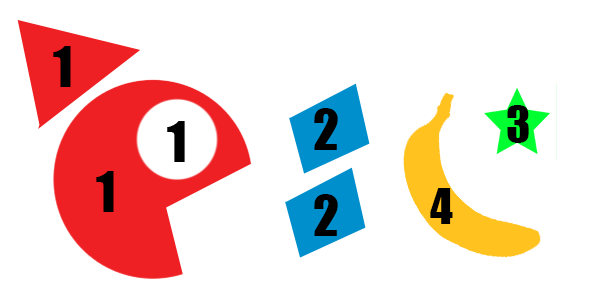
\includegraphics[width=\linewidth]{img/schemamergerA.png}
        \caption{Représentation des \texttt{Shapes} \{<1,1,1>,<2,2>,<3>,<4>\}}
    \end{subfigure}%
    ~ \\
    \begin{subfigure}{.7\linewidth}
        \centering
        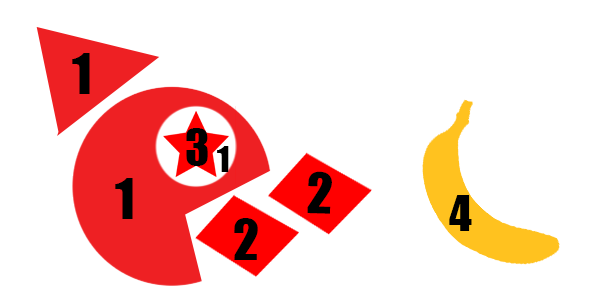
\includegraphics[width=\linewidth]{img/schemamergerB.png}
        \caption{Fusion des \texttt{Shapes} 1, 2 et 3}
    \end{subfigure}
    
    \caption{Fusion des groupes de \texttt{Shapes}: \{<1,1,1,2,3,3>,<4>\}}
    \label{fig:schemamerger}
\end{figure*}



Les deux classes Transformer et Merger ont été séparées car l'exécution du Merger est indépendante de celle du Transformer choisi. Cela permet également de simplement modifier la configuration de départ d'un algorithme en ne faisant aucun appel à Merger.


\paragraph{Solvers}

La classe \texttt{Solver} est également abstraite, son rôle est d'appliquer un algorithme de résolution sur la totalité des formes.\\
Elle contient les méthodes virtuelles \texttt{preSolve} et \texttt{solveBin}, qui permettent respectivement d'effectuer le traitement préliminaire nécessaire au bon fonctionnement du \texttt{Solver} et d'appliquer l'algorithme de résolution sur une seule plaque (en utilisant un sous-ensemble des \texttt{Shapes}).\\
La méthode \texttt{solveBin} travaille sur une liste d'indices lui indiquant les formes qu'il reste à packer. Lorsqu'une forme est effectivement packée, son indice est retiré de la liste.\\
\texttt{soveBin} est appelée tant que la liste d'indices restants est non vide. Travaillant à chaque fois sur une nouvelle plaque.  
L'algorithme appliqué dépend du \texttt{Solver} choisi (Scanline, Proba, ...).\\

Les tranformations faites par un \texttt{Solver} sont appliquées en place sur le \texttt{Layout} passé en paramètre à \texttt{Solver}, lequel est copié uniquement en cas d'exécution parallèle de plusieurs \texttt{Solvers} comme c'est le cas dans le \texttt{TaskSolver}.







\subsubsection{Outer}

La dernière étape de l'exécution a pour objectif d'écrire un fichier SVG contenant toutes les formes sélectionnées par l'utilisateur, après leur traitement par la classe \texttt{Solver}. Ceci est réalisé par la classe \texttt{Outer}, qui, à partir des formes précédemment déplacées par le \texttt{Solver} et de leurs identifiants récupérés par la classe \texttt{Parser}, va recopier les éléments associés à ces identifiants sur la sortie standard. \\

On parcourt donc l'arborescence du fichier SVG, en utilisant \texttt{rapidXML}, de manière à sélectionner les éléments en fonction de leur identifiant, pour ensuite ajouter un champ contenant la matrice de transformation associée aux déplacements effectués lors du packing (ou de modifier si le champ existe déjà).

La représentation obtenue au format SVG est alors stockée sous forme de chaîne de caractères dans un attribut de l'instance associée. %seems better 

Dans le cas d'une duplication (en bas de page), tous les éléments de l'arborescence parsés lors du parcours sont d'abord recopiés sans être modifiés. 
Les formes sont ensuite regroupées par plaques, en utilisant leurs coordonnées.
Ces groupes sont ensuite écrits dans le format SVG sur la sortie standard qui sera récupérée par le plugin ou par l'utilisateur pour être écrite dans un fichier.


%SCHEMA OUTER ICI
\subsection{Langage de script}
Tous les algorithmes précédemment évoqués sont dans des classes. Cela signifie que pour exécuter certains algorithmes dans un certain ordre, il fallait à l'origine instancier chacune des classes et appeler les bonnes méthodes sur ces derniers, imposant de recompiler le projet pour tout changement dans cet ordre ou dans les paramètres passés aux algorithmes.\\

Le temps de compilation du projet étant tout sauf instantané, il nous est apparu qu'il était nécessaire d'avoir une solution permettant de définir cet ordre à l'exécution plutôt qu'à la compilation. Nous avons alors eu l'idée d'introduire un langage de script extrêmement minimaliste permettant simplement de définir un ordre d'exécution ainsi que de passer des paramètres aux algorithmes.\\

Plutôt que de réaliser un parser ad-hoc pour ce nouveau langage, nous avons préférer le définir sous la forme d'une grammaire, et se reposer sur le module \texttt{Qi} de la librairie \texttt{Boost Spirit}, qui permet de construire des parsers basés sur une grammaire définie entièrement en C++, ce qui permet d'éviter une étape supplémentaire du type \texttt{yacc}n grâce à une redéfinition habile de multiples opérateurs.\\

Nous voulions comme fonctionnalités de base l'appel d'un \texttt{Solver} ou d'un \texttt{Transformer} avec des paramètres potentiels, ainsi que la possibilité de répéter des blocs d'instructions. Nous sommes alors arrivé à la grammaire fournie en annexe.\\

On constate qu'une instruction est alors toujours de la forme
$$\texttt{Fonction(param1=valeur1, param2=valeur2, ...);}.$$
et qu'on peut faire des blocs de telles instructions avec les mots-clés \texttt{BEGIN} et \texttt{END}, puis repéter de tels blocks avec la syntaxe \texttt{DO <X> TIMES <bloc>}.\\

\begin{figure}[H]
\centering
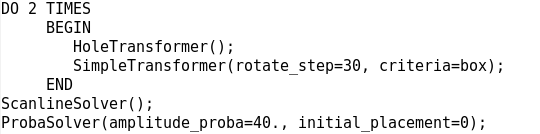
\includegraphics[scale=0.6]{img/closeEnough.png}
\caption{Un exemple de script}
\label{fig:closeEnough}
\end{figure}

On peut ainsi voir un exemple de script en figure~\ref{fig:closeEnough}. Dans ce dernier, on commence par exécuter \texttt{HoleTransformer}, puis \texttt{SimpleTransformer} (auquel on passe un entier et une chaîne de caractères), le tout deux fois. On appelle ensuite \texttt{ScanlineSolver} et \texttt{ProbaSolver}, auquel on passe un flottant et un entier.\\

À la manière de \texttt{yacc}, on associe à chaque règle un type et donc une valeur qui sera affectée à une instance de cette règle lors du parsing. On définit les actions grâce à une syntaxe spécifique à \texttt{Qi}. Nous avons choisi de stocker des informations basiques comme les noms, l'ordre, les paramètres des fonctions au fur et à mesure du parsing, et d'exécuter tout ce qui a été stocker à la fin de chaque \texttt{<big\_block>}.\\

Lors de l'exécution, il fallait associer à un nom de fonction dans le script une classe à instancier. Cela était au départ réalisé par une simple structure du type \texttt{if ... else if...}, mais quand le nombre d'algorithme a augmenté, nous avons voulu adopter une méthode plus générique.\\

Nous avons alors réalisé un mécanisme de registre, utilisant de manière intense la meta-programmation et les templates, permettant simplement d'instancier sur le tas une classe à partir de son nom et de lui transmettre les paramètres de l'utilisateur de façon entièrement automatique. Un registre est en fait un type disposant de méthodes statiques et se crée de la manière suivante :
$$\texttt{using NewReg = Registry<Base, boost::mpl::set<Derived1, Derived2, ...>::type>}$$

Les classes \texttt{Derived} devant hériter de \texttt{Base}. Toutes les classes doivent prendre en paramètre un ensemble de formes et un tableau de paramètres. Après la définition de ce nouveau registre, il faut initialiser sa table interne en appelant \texttt{NewRegistry::Init()} une unique fois. Il suffit ensuite pour instancier une classe depuis son nom d'appeler :
$$\texttt{NewReg::instanciate("Derived2", shapes, params)}$$
Cette fonction retourne un \texttt{Base*} contenant une instance de \texttt{Derived2}. De plus, les règles de la grammaire peuvent être écrites de manière automatique grâce à ce mécanisme (en exploitant le registre, qui contient en interne une \texttt{map} entre chaînes de caractère et pointeurs sur fonction).\\

Ainsi lorsqu'on veut ajouter un \texttt{Solver} ou un \texttt{Transformer} à la grammaire, il suffit seulement d'ajouter son type à la définition du registre, et tout le reste est généré automatiquement. Nous obtenons donc un langage de script très facile à étendre.\\

Pour exécuter nos algorithmes, il ne reste alors qu'à appeler le parser généré depuis le \texttt{main}, et tous les algorithmes sont exécutés au cours du parsing.
    